\section{Additional Results and Diagnostics}
\label{app:additional}
\setcounter{equation}{0}
\setcounter{table}{0}
\setcounter{figure}{0}

\subsection{Data Characterization and Effective Rank}

\subsubsection{Modality-to-Target Kernel Alignment}

Figure~\ref{fig:data-characterization}(a) uses RBF centered-kernel alignment (CKA), implemented as centered normalized HSIC, as a data-level dependence proxy between each input modality and either the low-pass background or structural complement. Within each OpenFWI subset, each representation is flattened; modality representations are divided by the square root of their feature count, and the RBF bandwidth is the median non-zero pairwise Euclidean distance for that representation. The plotted summary uses the median CKA over the eight subsets. A fixed seeded permutation of target rows provides the shuffled control. The resulting CKA values characterize modality-to-target alignment.

\subsubsection{Participation-Ratio Effective Rank}

For the descriptive decomposition $V=B+S$, with $B=P_L(V)$ and $S=V-B$, participation-ratio effective rank is
\begin{equation}
r_{\mathrm{eff}}=
\frac{\left(\sum_j\lambda_j\right)^2}{\sum_j\lambda_j^2},
\end{equation}
where $\{\lambda_j\}$ are nonzero covariance eigenvalues. The analysis uses 1,000 fixed training records per OpenFWI subset and no learned dimensionality reducer.

\begin{table}[H]
\centering
\caption{Participation-ratio effective rank of the chosen low-pass background and structural complement.}\label{tab:appendix-rank}
\begin{tabular}{lrr}
\toprule
Subset & Background $B$ & Structure $S$ \\
\midrule
FlatVel-A & 2.02 & 24.26 \\
FlatVel-B & 5.66 & 39.67 \\
CurveVel-A & 2.59 & 58.52 \\
CurveVel-B & 7.53 & 200.89 \\
FlatFault-A & 3.06 & 37.83 \\
FlatFault-B & 7.54 & 289.69 \\
CurveFault-A & 4.24 & 49.54 \\
CurveFault-B & 10.54 & 407.91 \\
\midrule
Median & 4.95 & 54.03 \\
\bottomrule
\end{tabular}
\end{table}

The structural complement has higher effective rank in every subset, characterizing the distribution of variation under the selected low-pass decomposition.

\subsection{Sensitivity to Observation Removal}

A fixed trained BG-RFM model is evaluated without retraining after removing individual observations or observation groups. Removal is implemented in two coordinated steps: the corresponding observation tensor is replaced/zeroed, and its availability/quality mask state is updated so the routing mechanism does not treat the removed observation as available. Because the model is trained under full multimodal input, this test measures input-removal sensitivity under distribution shift rather than isolated causal modality contributions.

The full-input results are reported in Table~\ref{tab:rs-main}.

\begin{table}[t]
\centering
\caption{Sensitivity to observation removal without retraining or test-time adaptation.}\label{tab:appendix-observation-removal}
\begin{tabular}{lrrr}
\toprule
Observation subset & MAE & RMSE & SSIM \\
\midrule
w/o well log & 0.0168 & 0.0295 & 0.9899 \\
w/o horizon & 0.1011 & 0.1669 & 0.8202 \\
w/o RMS velocity & 0.3947 & 0.4705 & 0.0753 \\
w/o well log + RMS velocity & 0.4684 & 0.5303 & 0.0192 \\
PSTM only & 0.4706 & 0.5356 & 0.0154 \\
\bottomrule
\end{tabular}
\end{table}

Removing RMS velocity or horizons produces larger reconstruction changes than removing the sparse well channel in this evaluation.

\subsection{Condition and Transport Diagnostics}

Cross-modal retrieval is measured in the role-projected embedding spaces using symmetric Recall@1: within fixed same-subset galleries of complete-modality records, a query from one modality retrieves keys from another modality, the correct match is the same record, and the two retrieval directions are averaged. The diagnostic uses galleries of 128 records, ten galleries per subset, with gallery seed 42.

Anchor similarity is the cosine similarity between an $\ell_2$-normalized role-projected modality representation and the corresponding normalized projected training-time anchor, averaged over available modalities for each record. The deranged control applies a strict one-row cyclic derangement with no fixed points. The reported anchor margin is the per-record matched-minus-deranged difference.

Role specialization uses the fused conditions. With the same $5\times5$ low-pass operator, $\eta_B$ is the low-frequency magnitude ratio of $C_{\mathrm{bg}}$, $\eta_S$ is the high-frequency magnitude ratio of $C_{\mathrm{str}}$, and $\chi_{BS}$ is the absolute cosine similarity between adaptively pooled background and structural condition vectors.

For anchor-margin uncertainty, 95\% bootstrap intervals are obtained from 1000 resamples with replacement of the per-record matched-minus-deranged differences; the displayed interval endpoints are the 2.5th and 97.5th percentiles. The background and structural bootstrap seeds are 17 and 29, respectively.

For the transport diagnostic, the unit-variance Gaussian base contributes one unit of expected squared energy per state dimension. The resulting Gaussian-base-averaged straight-path target-energy ratio is
\begin{equation}
q_T=
\frac{d^{-1}\|V-\hat B\|_2^2+1}
{d^{-1}\|V\|_2^2+1},
\qquad d=HW .
\end{equation}
All 33,600 held-out samples satisfy $q_T<1$ in the evaluated analysis; the mean is 0.772 with bootstrap 95\% confidence interval $[0.771,0.773]$. This interval is obtained by 2000 sample-level bootstrap resamples of the per-record $q_T$ values using seed 2027. This quantity characterizes the background-centered transport target in the evaluated normalized coordinates.

\begin{figure}[t]
\centering
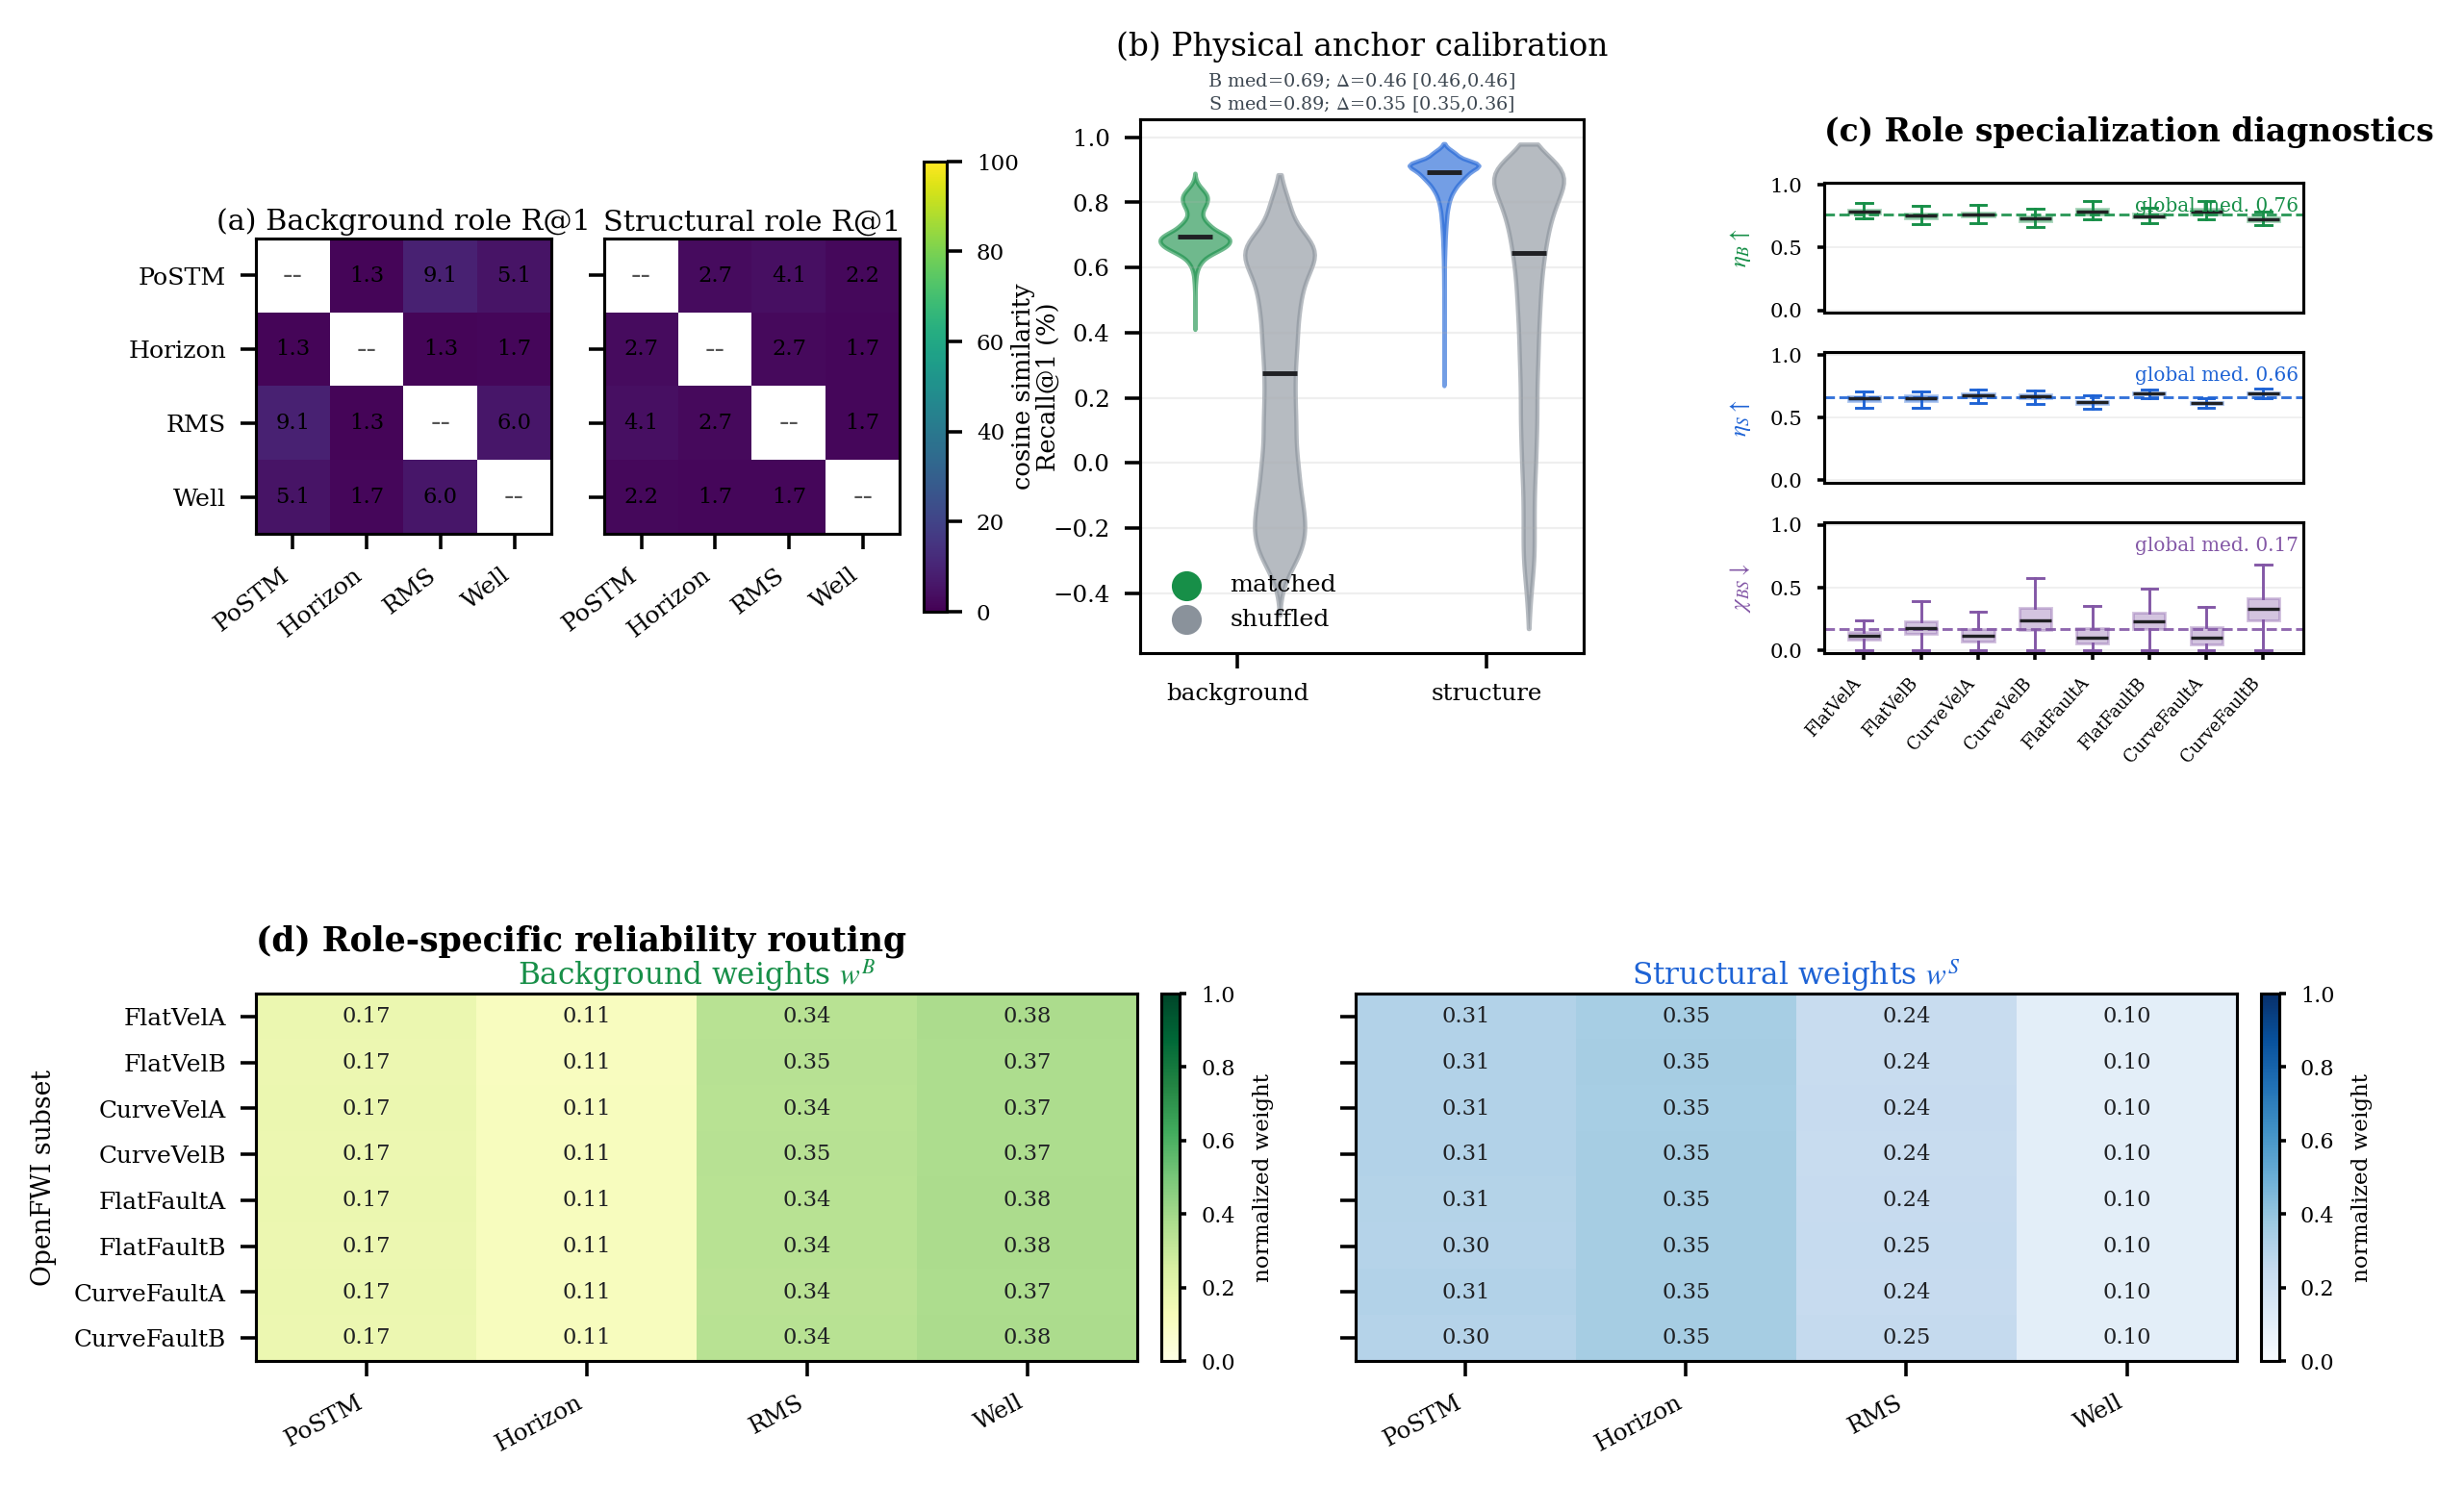
\includegraphics[width=0.95\textwidth]{../AAAI2027/figures/figure3_condition_learning/appendix_full_condition_diagnostics.png}
\caption{Extended condition-routing diagnostics. Cross-modal retrieval uses symmetric Recall@1 in role-projected spaces; anchor calibration compares matched and strictly deranged anchor similarities; role-specialization statistics describe the fused conditions; routing weights are post-training encoder outputs. These quantities characterize the learned role interfaces.}\label{fig:appendix-condition-routing}
\end{figure}

\subsection{Additional Qualitative Cases}

The additional panels follow the performance-dependent SSIM selection rule specified in Section~\ref{sec:results-qualitative}; negative-margin cases are included separately.

For the composite appendix panels, embedded legacy labels map to the manuscript terminology as follows:
\begin{itemize}
    \item PD-BG-RFM $\rightarrow$ BG-RFM;
    \item InversionNet $\rightarrow$ InversionNet adaptation;
    \item VelocityGAN $\rightarrow$ VelocityGAN adaptation;
    \item UPFWI $\rightarrow$ UPFWI-derived supervised multimodal backbone;
    \item Latent U-Net (Large) $\rightarrow$ Latent U-Net adaptation;
    \item Auto-Linear denotes an additional adapted baseline that is not included in the main comparison table.
\end{itemize}

\begin{figure}[t]
\centering
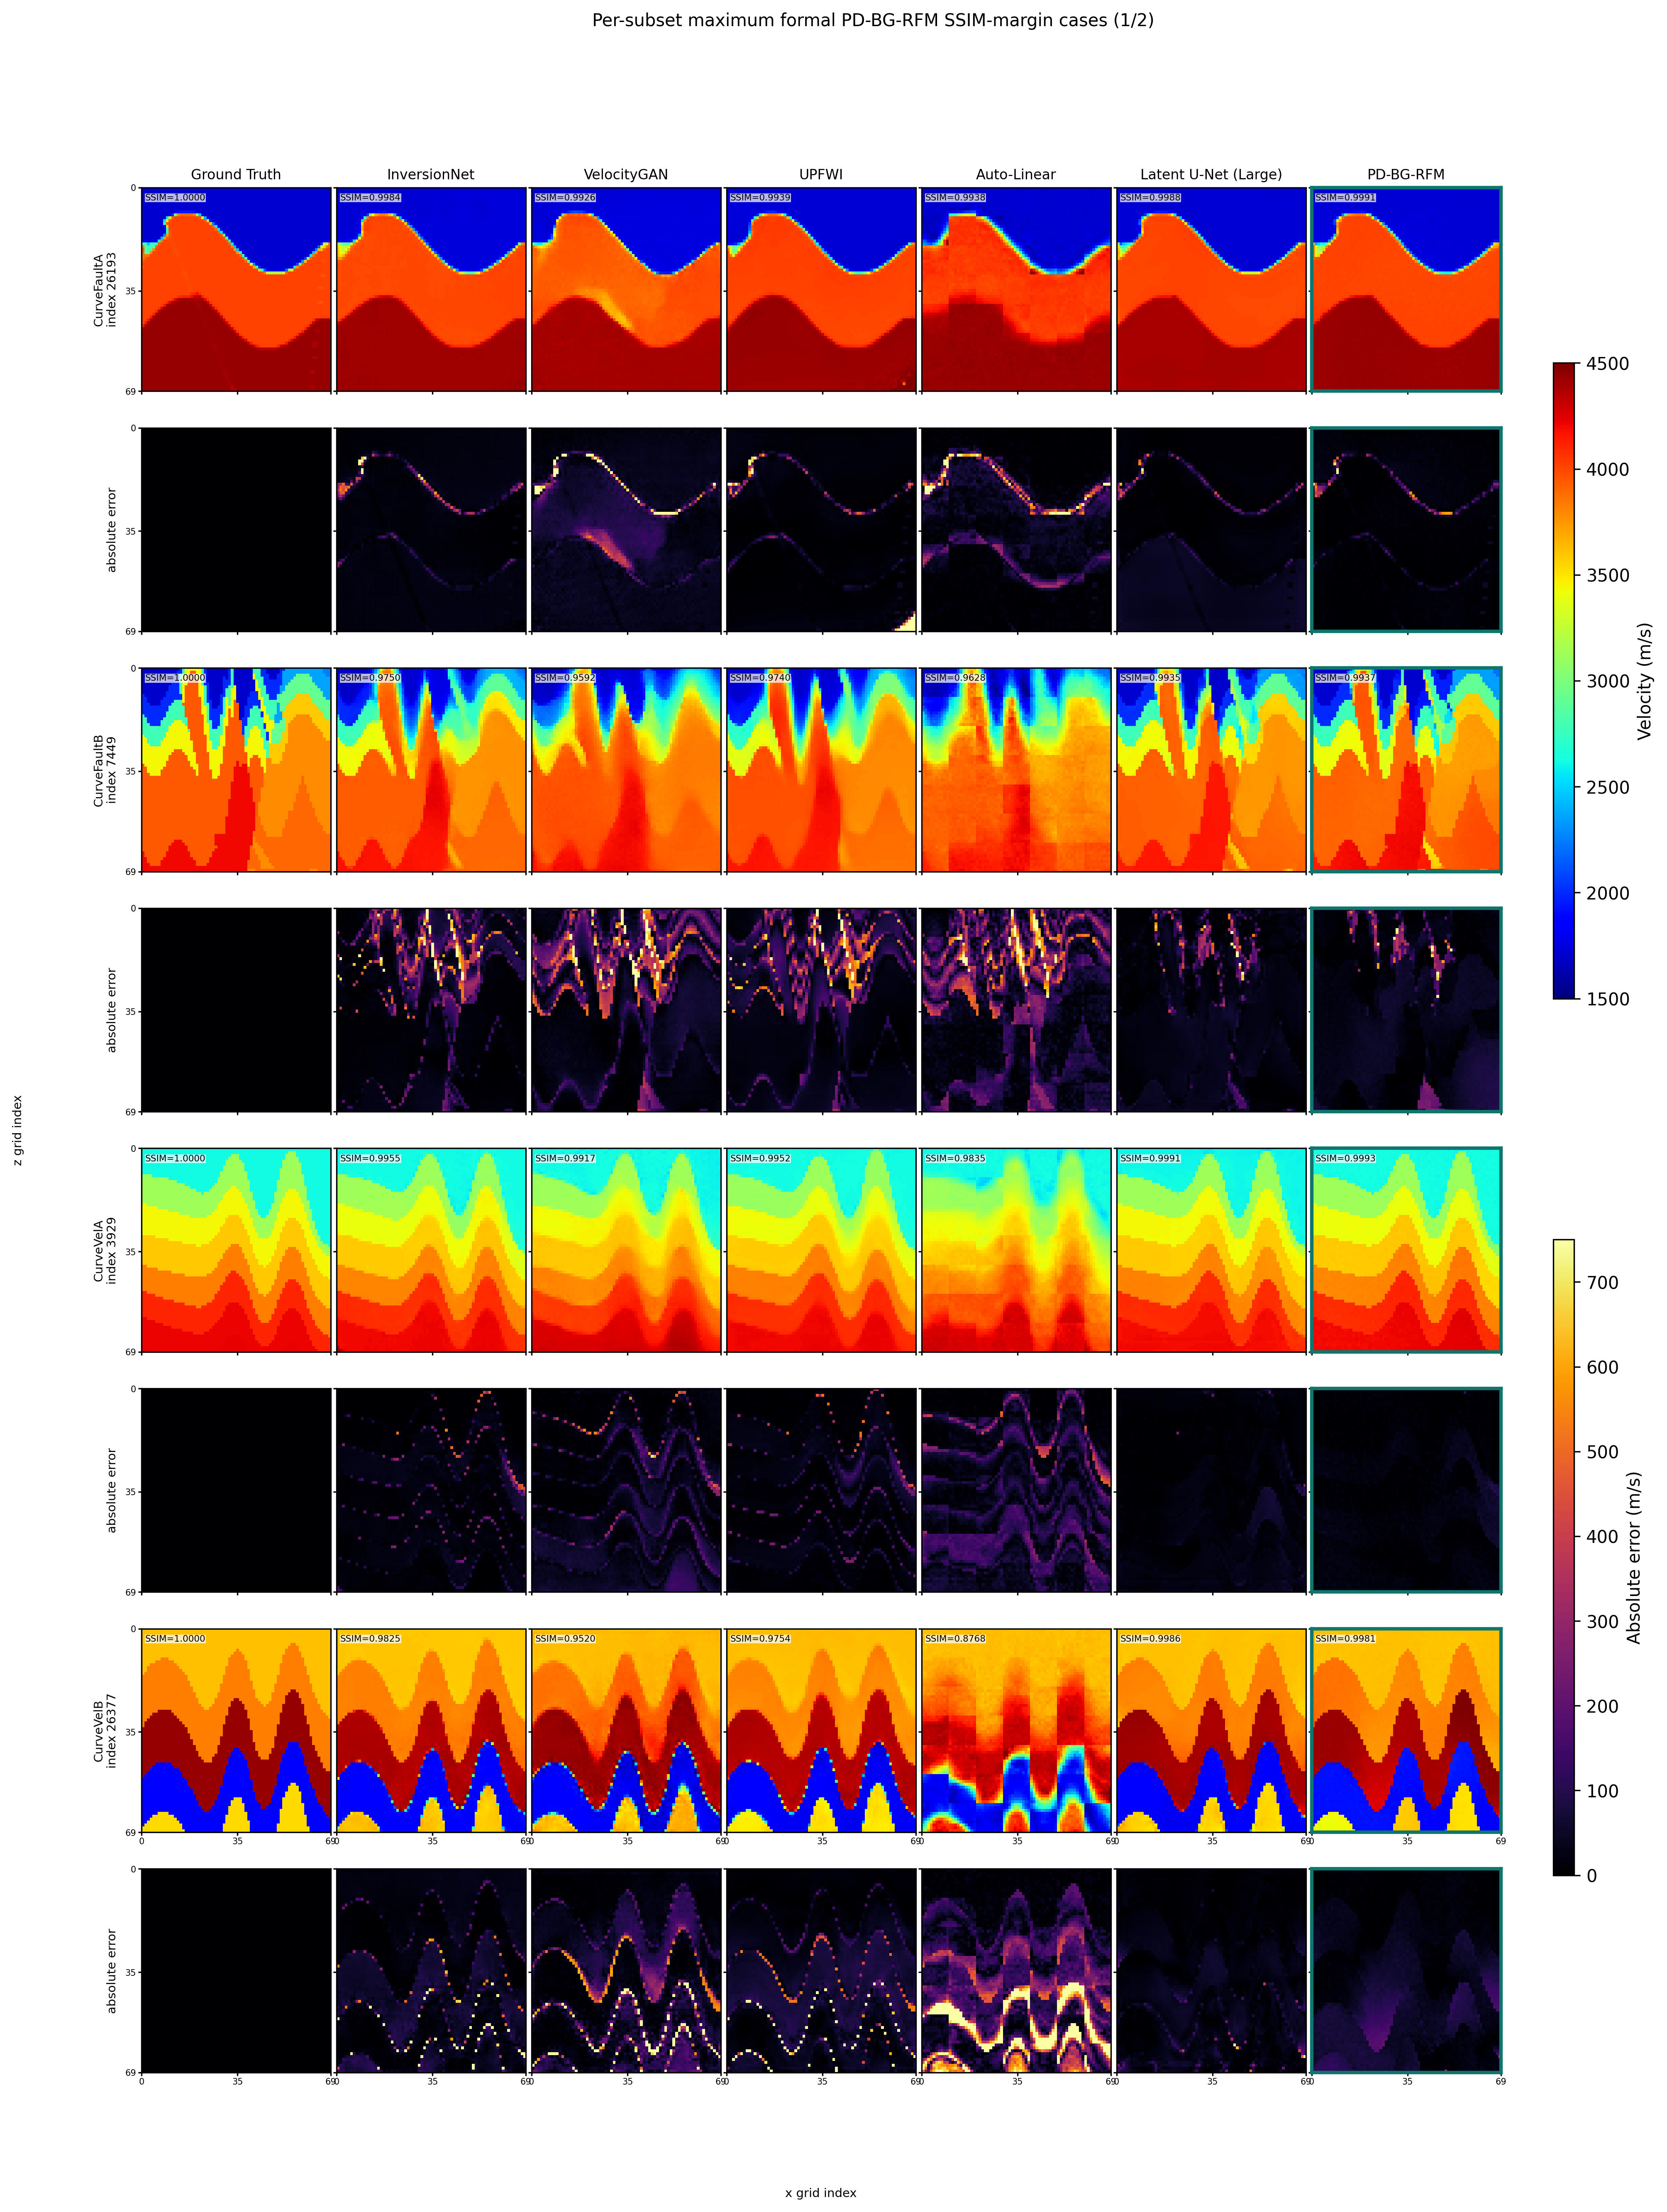
\includegraphics[width=0.98\textwidth]{../AAAI2027/figures/table2_qualitative/table2_representative_cases_1.png}
\caption{Performance-selected per-subset maximum-SSIM-margin cases, part I.}\label{fig:appendix-selected-1}
\end{figure}

\begin{figure}[t]
\centering
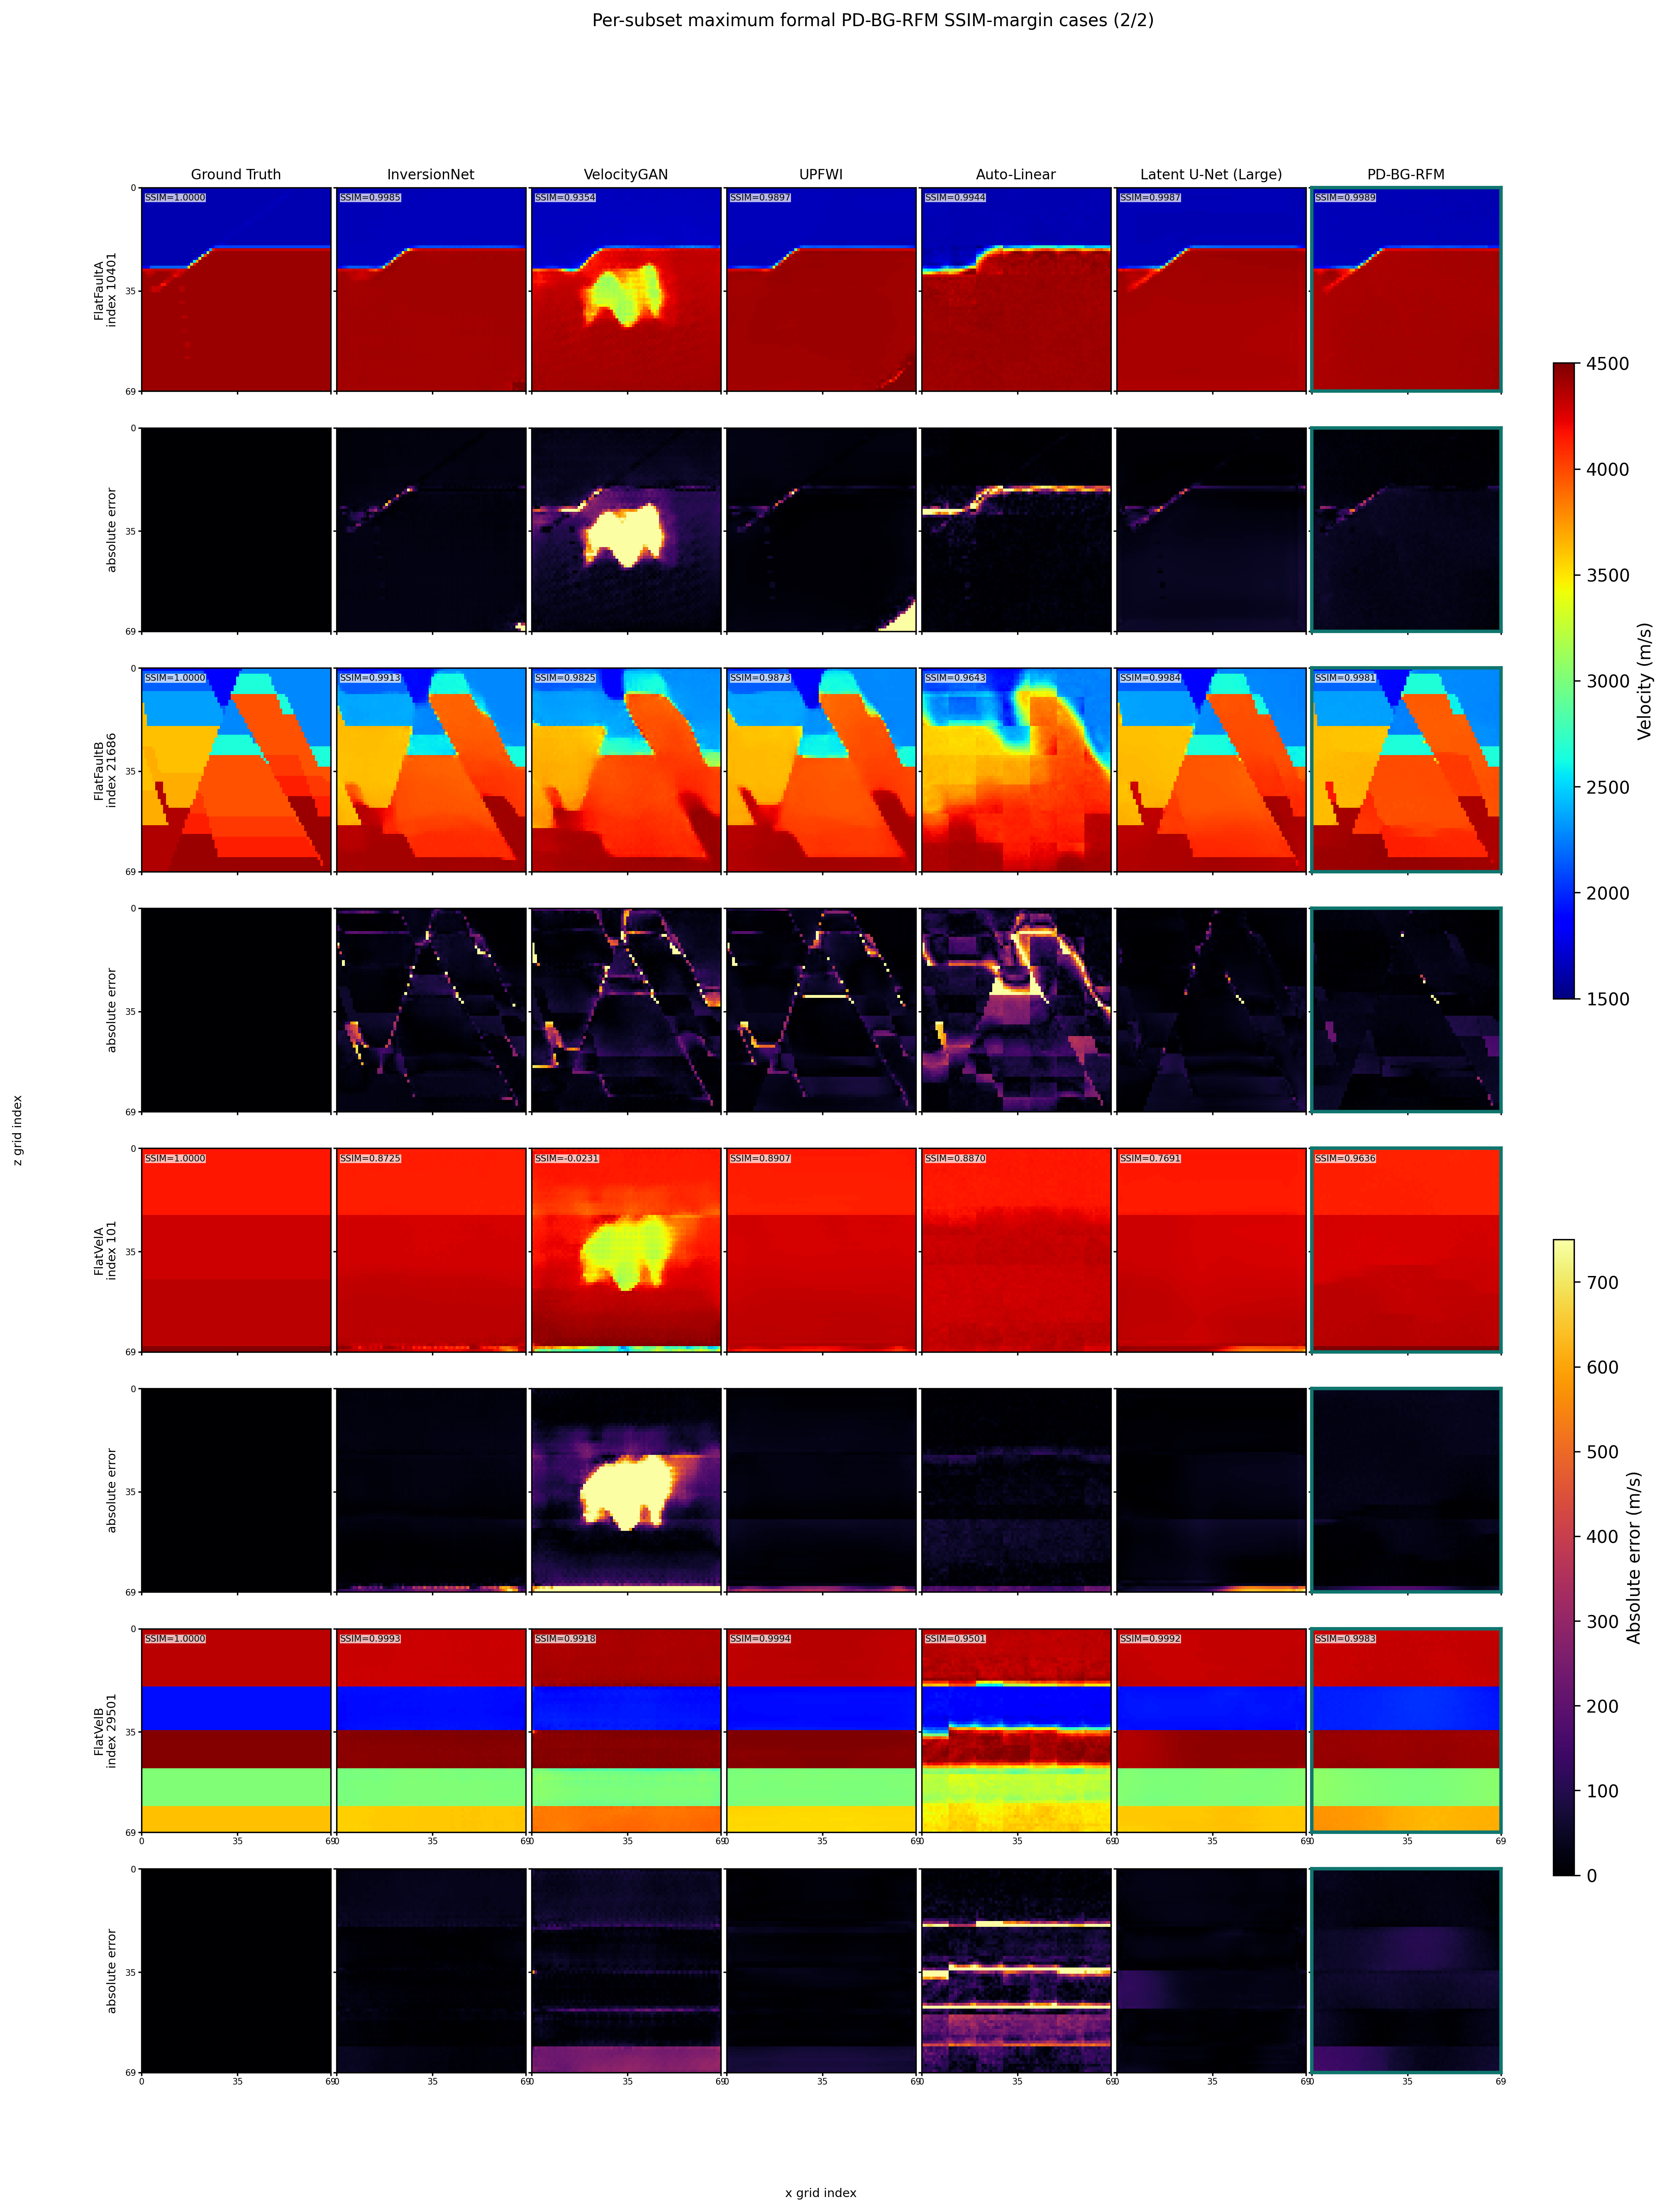
\includegraphics[width=0.98\textwidth]{../AAAI2027/figures/table2_qualitative/table2_representative_cases_2.png}
\caption{Performance-selected per-subset maximum-SSIM-margin cases, part II.}\label{fig:appendix-selected-2}
\end{figure}

\begin{figure}[t]
\centering
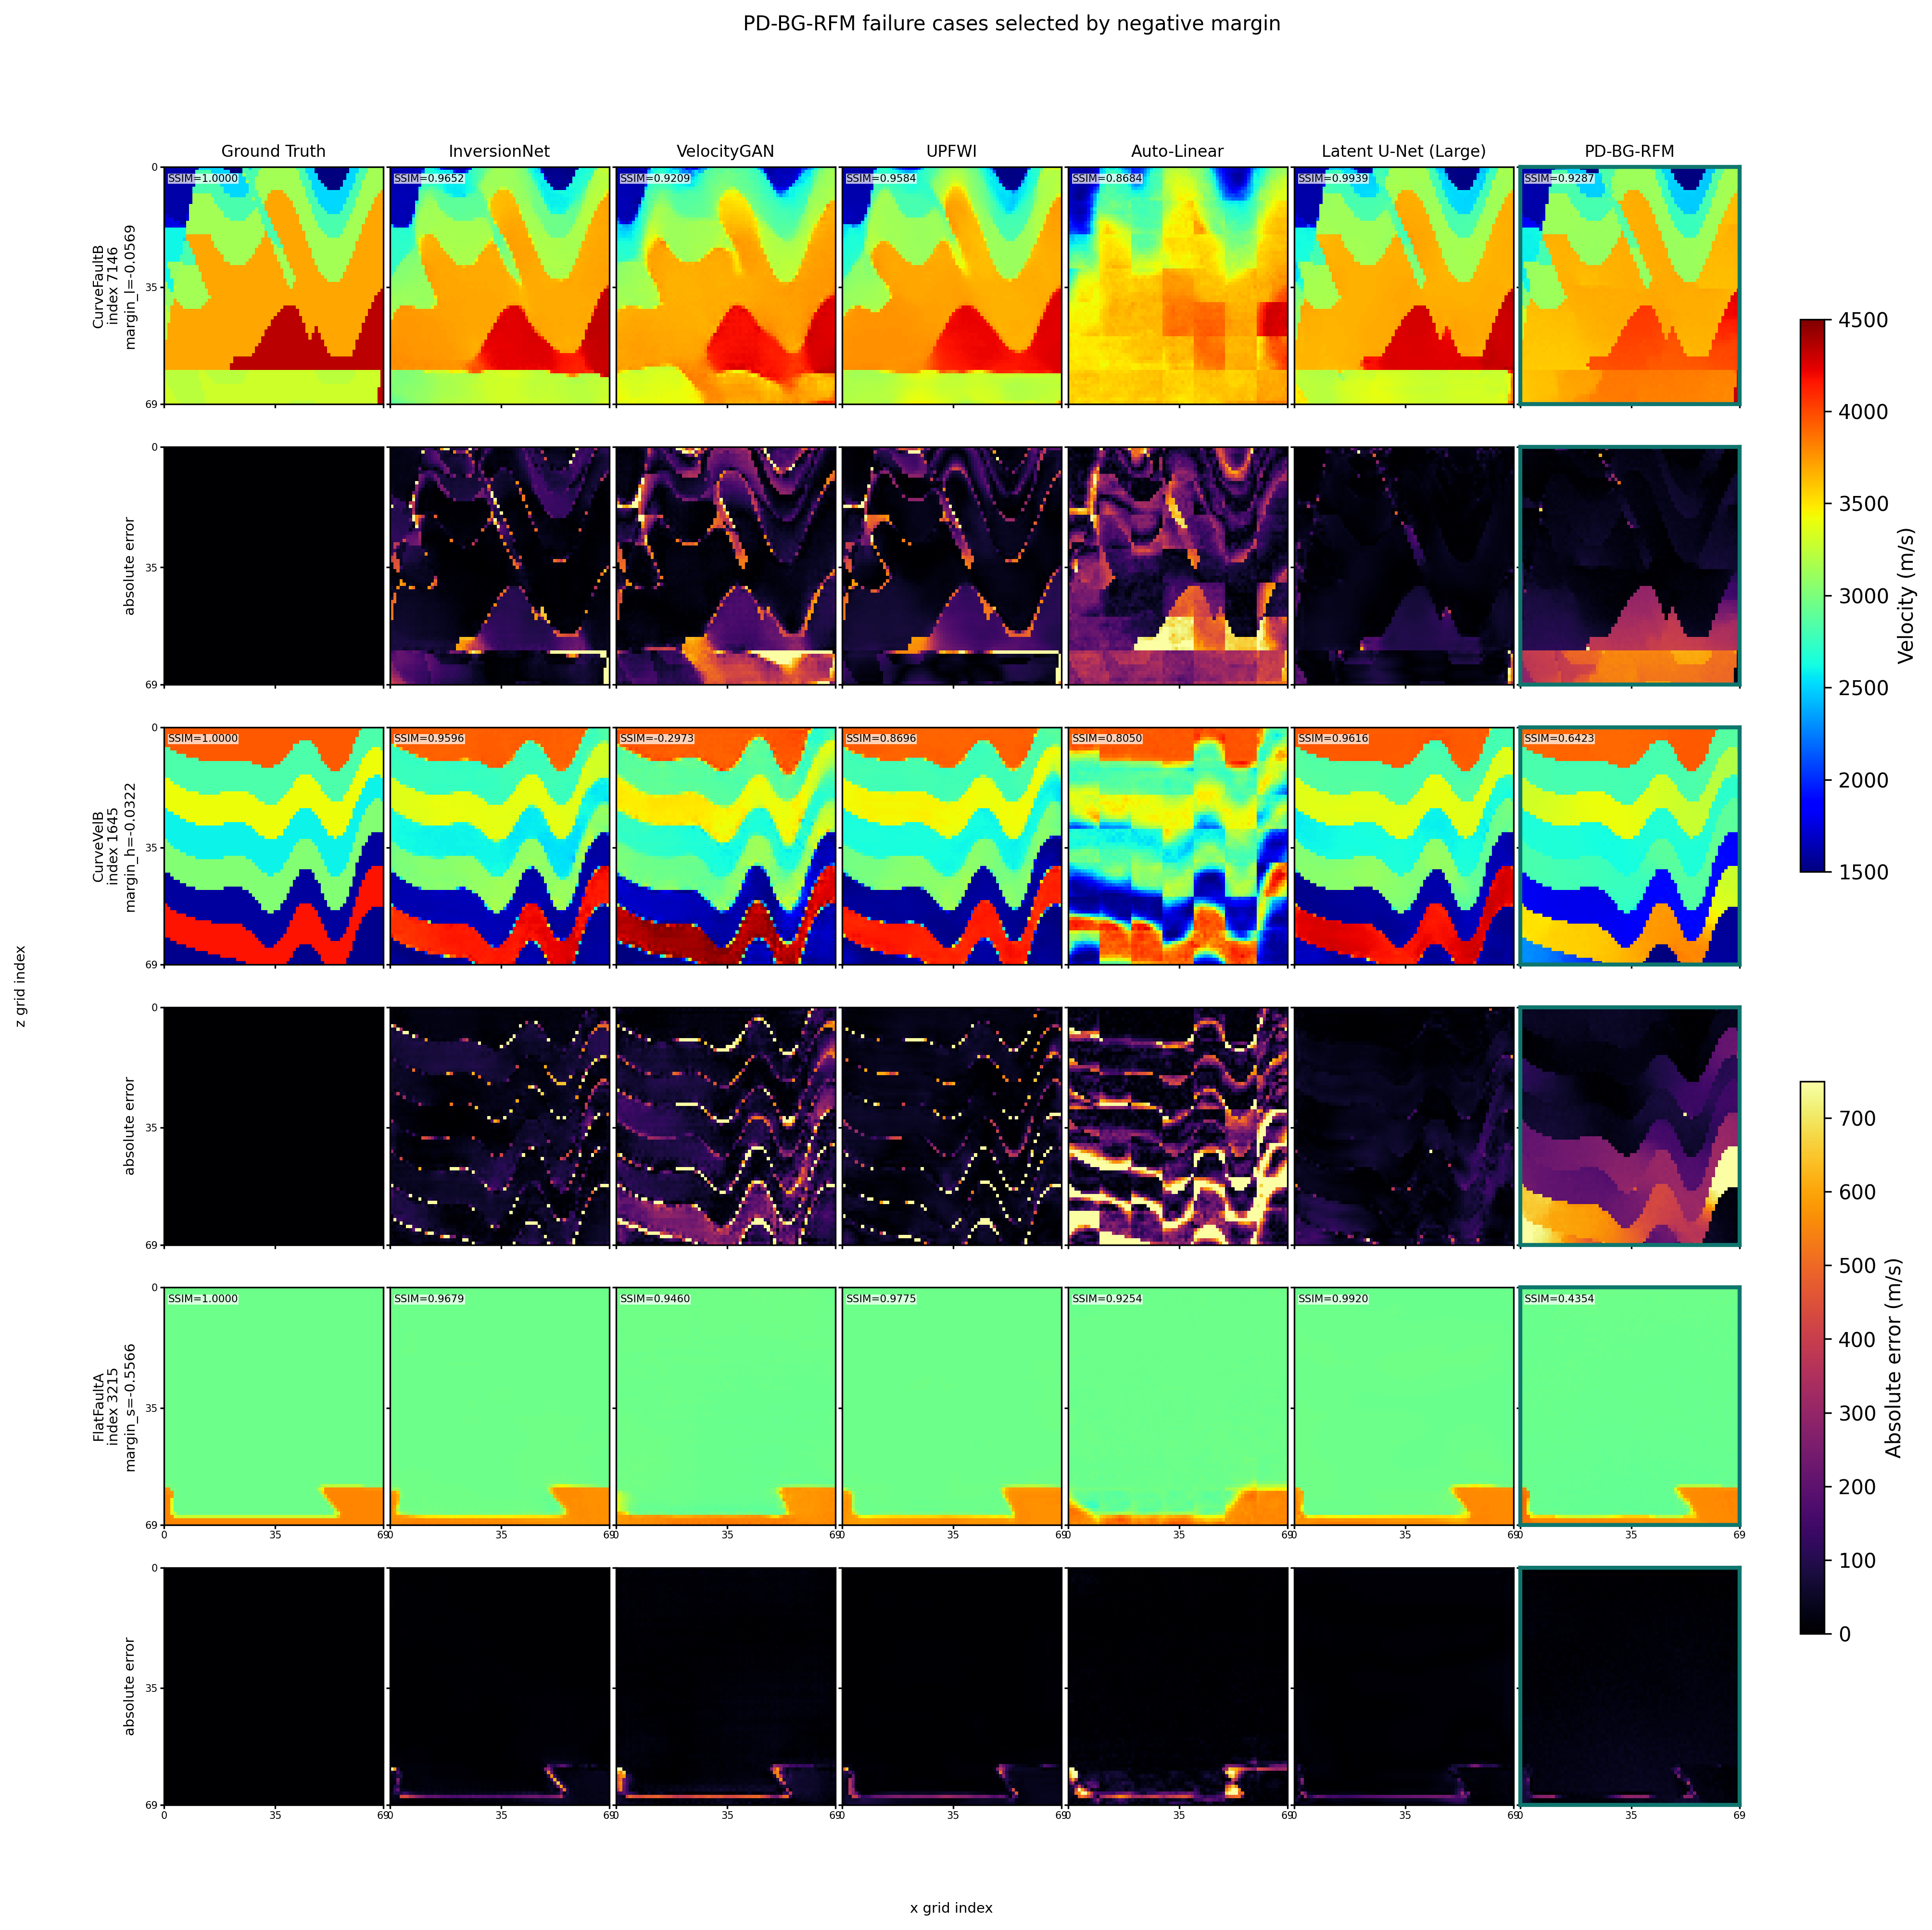
\includegraphics[width=0.98\textwidth]{../AAAI2027/figures/table2_qualitative/table2_failure_cases.png}
\caption{Failure cases selected by the most negative predefined low-frequency, high-frequency, and SSIM margins.}\label{fig:appendix-failure-cases}
\end{figure}
